\documentclass[tikz,border=10pt]{standalone}
\begin{document}
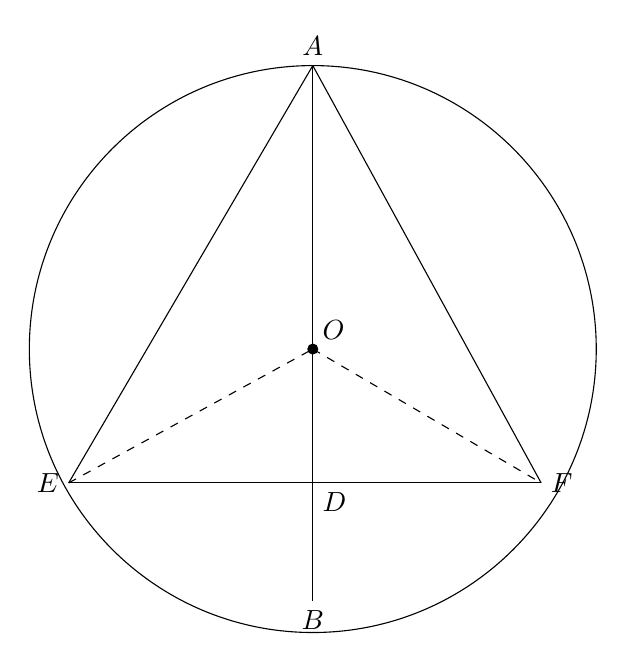
\begin{tikzpicture}[scale=1]

% Coordinates
\coordinate (O) at (0,0);
\coordinate (A) at (0,3.6);
\coordinate (B) at (0,-3.2);
\coordinate (D) at (0,-1.7);
\coordinate (E) at (-3.1,-1.7);
\coordinate (F) at (2.9,-1.7);

% Circle
\draw (O) circle[radius=3.6];

% Solid segments
\draw (A) -- (E);
\draw (A) -- (F);
\draw (A) -- (B);
\draw (E) -- (F);

% Dashed segments
\draw[dashed] (E) -- (O);
\draw[dashed] (O) -- (F);

% Point O
\fill (O) circle[radius=2pt];

% Labels
\node[above] at (A) {$A$};
\node[below] at (B) {$B$};
\node[above right] at (O) {$O$};
\node[below right] at (D) {$D$};
\node[left] at (E) {$E$};
\node[right] at (F) {$F$};

\end{tikzpicture}
\end{document}
